\chapter{System Overview}
\label{chap:overview}

In this chapter we present an overview of our system. 
We will start by providing an overall description of the system: 
the main components and how these relate to each other. 
This will be followed by the possible user interactions: 
the different types of queries that can be requested to our backend as well as how these requests are handled.

In this section we intend for readers to get a general overview of the work; we will go into finer detail for the individual components in \Cref{chap:Backend} and \Cref{chap:Frontend}.

\section{System Architecture}

Our system architecture is as depicted in \Cref{fig:architecture}.

\begin{figure}[H]
    \centering
        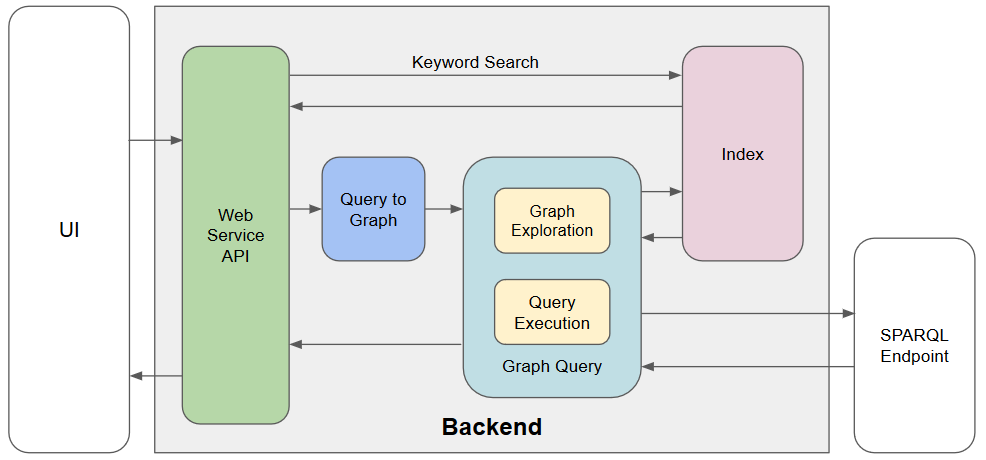
\includegraphics[width=\linewidth]{imagenes/architecture.png}
        \caption{System Architecture.}
        \label{fig:architecture}
\end{figure}

Our system allow users that are building SPARQL queries to get entity and property suggestions from a triplestore. 
This works in two ways: 
A first contribution is to allow users to query entities or properties via keyword search. 
The second and most important contribution of our work is to provide suggestions for SPARQL terms, based on the query that is being built. 
All given suggestions are sorted by relevance and importance.

Our system is built entirely as a web service backend. 
This backend sits between the user interface and a remote SPARQL query endpoint. 
The entry point of our system is an API that will take requests from different services, such as SPARQL query editors or SPARQL visual explorers. 

Depending on the query type, the system can do a keyword search directly on the index or it can parse the query for SPARQL triple patterns. 
In the latter case, the SPARQL query will be converted to a graph. 
This graph will be processed and then sent for execution. 
The execution of the query is sent in parallel to both the remote SPARQL endpoint and the local index. 
The results are then post-processed and sent back to the user for display and selection. 
We will expand some more on this steps in the following sections.

These last interactions, related to the UI, are not in the scope of our work; nevertheless, we have integrated our system to a visual query system for demonstration. 
This UI integration, both for the request and the display of results, is explained in detail in \Cref{chap:Frontend}.

It is important to mention that before our system can provide results, it has to be initialized with an RDF dataset dump. 
This initialization process can be divided into two sub-processes: 
Pre-processing and Indexing. 
The details of this initialization are described in \Cref{chap:init}. 

All of the source code for the back-end is written in \textit{C\#} as a .Net Standard Library. 
The following dependencies are used:

\begin{itemize}
    \item \textit{Lucene.Net}\footnote{\url{https://lucenenet.apache.org}} is used for the index. 
    \item \textit{DotNetRDF}\footnote{\url{https://www.dotnetrdf.org}} is used for handling, reading and writing RDF.
    \item \textit{SharpZipLib}\footnote{\url{http://icsharpcode.github.io/SharpZipLib}} is used for handling compression.
    \item \textit{Mime}\footnote{\url{https://github.com/hey-red/Mime}} is used for identifying file types checks.
    \item \textit{xUnit}\footnote{\url{https://xunit.net}} is used for Unit Testing.
    \item \textit{NLog}\footnote{\url{https://nlog-project.org}} is used for logging.
    \item \textit{ASPNetCore}\footnote{\url{https://docs.microsoft.com/en-us/aspnet/core}} is used for the Application Interface (API).
    \item \textit{Newtonsoft.Json}\footnote{\url{https://www.newtonsoft.com/json}} is used for handling JSON.
\end{itemize}

The integration code for the front-end is written in \textit{Javascript}. The code is available at the following locations:
\begin{itemize}
    \item \url{https://github.com/gabrieldelaparra/SPARQLforHumans}. This project.
    \item \url{https://github.com/gabrieldelaparra/RDFExplorer}. Forked and modified version of RDFExplorer.
    \item \url{https://github.com/hvarg/RDFExplorer}. RDFExplorer~\cite{Vargas2019}.
\end{itemize}

\section{User Interactions}

As mentioned before our system has two different ways for users to request information: 
Keyword search 
and SPARQL query term suggestions.

\subsection{Keyword search}

The keyword search feature enrich the user experience of RDF datasets by providing lookup access via \textit{labels}, \textit{descriptions} or \textit{alternative labels} for the queried data. 
Keyword search functionality is one of the most natural ways of looking for information. 
While this feature is the de-facto way for users to search for something (e.g. DuckDuckGo) it is not included as part of the SPARQL standard. 
Keyword search allows users with no or limited knowledge of prefixes or ids to get to their desired results. 
The keyword search mechanics are quite straightforward; a keyword request is sent to the backend and a list of possible entities or properties, sorted by relevance, are returned. 

\begin{example}
A user wants to search for the type \textit{Human} in the Wikidata dataset. 
They could have no idea that \textit{wd:Q5} is the identifier for this entity. 
They could search for \textit{"person"} or \textit{"people"} instead. 
Since \textit{person} and \textit{people} are alternative labels for \textit{Human}, the latter is displayed in the results. 
As per the results, \textit{Human} is displayed before \textit{Grammatical Person}, since human is deemed to be more likely to be of relevance to the user, and thus is given a higher order than what the alphabetic order would sort.
\end{example}

\begin{example}
A user would like to search for the \textit{head of government (wdt:P6)}  property, once again, in the Wikidata dataset. 
As keywords, the user could enter \textit{"president"}, \textit{"mayor"} or \textit{"prime minister"}, since this would be a more natural way of looking for that property, depending on the user and query context. Once again, suggestions including \textit{head of government} are returned and ordered by a measure of how likely they are to be relevant to the user.
\end{example}

\begin{example}
A user is trying to search for \textit{Reykjavík}. 
Since typing the name correctly would be a challenge for certain users, this author included, the \textit{"capital (of) Iceland"} could be used to search. 
Since the system has been indexed for \textit{descriptions}, the desired result would appear as the first result. 
\end{example}

\subsection{SPARQL query term suggestions}

The term suggestions help users to create SPARQL queries. 
A SPARQL query is composed of multiple triple patterns.
As seen in \Cref{chap:SPARQL}, a triple pattern can be something like \textit{"Mary eats pizza"}. 
Lucky Mary. 
Each triple in the SPARQL grammar is composed of three terms: 
a \textit{subject} (\textit{"Mary"}), 
a \textit{predicate} (\textit{"eats"}) 
and an \textit{object} (\textit{"pizza"}). 

We will now briefly describe this process' overview; the details will be revised in more detail in \Cref{chap:Backend}. 
We will accompany this description with some examples about the delicious pizza Mary was eating.

Query construction starts by supposing that a triple pattern is always available, even when there are only variables, such as in \textit{?var1 ?prop1 ?var2}. However, triple patterns will often contain specific terms in combination with variables, as seen in the previous example.

As a first step, an application uses our service for getting suggestions. 
The user of this application still has not added anything to its query. 
For a blank string, a triple pattern with only variables is added. 
The following triple pattern represents the current query:

\begin{minted}[escapeinside=||,frame=none,linenos=false]{text}
    ?var1 ?prop1 ?var2 .
\end{minted}

During query construction, a user will start adding terms to their triple patterns. 
At this stage, if everything is a variable, the keyword search will return results. 
In this context, a user might start by typing \textit{"Ma"} and several suggestions will be displayed. 
For this example, the results will include \textit{"Mary"}, \textit{"Marocco"} or \textit{"Mango"}. 
The user selects \textit{"Mary"} between the suggestions and \textit{Mary} is added to the query as the \textit{subject} term. 
The system recognizes that \textit{Mary} is of type \textit{Human}. The triple should now look like this:

\begin{minted}[escapeinside=||,frame=none,linenos=false]{text}
    |\bf{Mary}| ?prop1 ?var2 .
\end{minted}

Next the user moves to the \textit{predicate} \texttt{?prop}. 
The user will get suggestions like \textit{"eats"}, \textit{"parent of"} or \textit{"studies at"}, which are defined on subjects of type \textit{Human} in the data, but not \textit{"capital of"}, which is not defined on any subject of type human in the data. 
The user selects \textit{eats}. The predicate is replaced with that property. 
The query at this stage looks like:

\begin{minted}[escapeinside=||,frame=none,linenos=false]{text}
    |\bf{Mary}| |\bf{eats}| ?var2 .
\end{minted}

Next the user moves to the \textit{object}, which is a variable. 
Several suggestions like \textit{"cake"}, \textit{"tofu"}, etc. are displayed. 
The user can type in \textit{"pi"} and will be suggested \textit{"pie"}, \textit{"pizza"}, \textit{"pineapple"}, etc., but not \textit{"pillow"} or \textit{"pictures"}, etc., as these are not eaten by anything in the data, nor \textit{"pine cones"}, \textit{"pigeons"}, etc., which though eaten in the data are not eaten by instances of \textit{Human}.

This process might continue until the user has finished building the query. 
At any stage the user can leave a term as a variable and query for all the values that the variable takes.
The user can also join statements, creating more complex queries.

Behind the curtains, during this query construction process the input data is read from the SPARQL query, parsed and stored into a data structure for further processing. 
Our system will convert that query into a graph. 
More about the conversion between SPARQL query and such graphs will be covered in \Cref{chap:parser}.

This graph will be then explored to check for relations between the nodes and the edges. 
Each of the nodes and edges will be classified as either variables, given types or inferred types. 
If other statements are given at this stage, a decision process involving given-types and intersections between inferred types for different incoming/outgoing properties would occur. 
This helps the system to correctly assign types based on the explicitly given ones and the inferred ones. 
All of this will be covered in more detail in \Cref{chap:graph_exploration}.

Once all nodes and edges have been classified, the information will be requested in parallel threads from both sources: 
Local Index and Remote SPARQL Endpoint. 
The request to the remote endpoint is sent with a configurable timeout, usually of a few seconds. 
If the remote endpoint returns values within this time, this results will be returned; otherwise, our internal local index results will be returned. The local results will only be returned if the remote endpoint request fails/times-out. 
This double request mechanism allow us to suggest possible results that would otherwise keep the user indefinitely waiting or in the worst case, never return. 
More on this in \Cref{chap:execution}.

Once the results are consolidated, they will be returned to the UI which made the request. 
For testing purposes, we have integrated our system within an existing visual SPARQL building frontend. 
This integration is described in \Cref{chap:Frontend}.

Before ending this chapter, we would like to emphasize something that was mentioned before. 
Our system can provide approximate results for some triple patterns in complex queries. 
We will try to explain these approximations by example. 
Consider that in our input dataset, there is no such triple for Mary (Mary eats Pizza), but that triple does exist for Bob (Bob eats Pizza). 
While constructing a complex query, where the remote endpoint times out, the local index results for a instance of type \textit{Human} and for the \textit{eats} predicate, will return Pizza as one of the alternatives.
This is due to the nature of our index.
Our index is not based on complete triples, but types, domains and ranges.
This way of indexing supports the query term suggestion tasks, but approximates results for such cases.